\documentclass[11pt,a4paper]{article}
\usepackage[utf8]{inputenc}
\usepackage[spanish]{babel}
\usepackage{amsmath, amssymb}
\usepackage{graphicx}
\usepackage{booktabs}
\usepackage{geometry}
\geometry{letterpaper, margin=1in}

\title{Reporte Automático de Optimización Numérica}
\author{Motor Híbrido C-Python (DE)}
\date{\today}

\begin{document}
\maketitle

\begin{abstract}
Este reporte describe la parametrización automática del Factor de Estructura Estático $S(q)$ para sistemas coloidales, procesando datos experimentales o de simulación extraídos directamente de observaciones recientes. Empleamos un pipeline híbrido con motor de cálculo en C y una capa de optimización global en Python soportada por el algoritmo de Differential Evolution (DE) extrayendo un análisis de los 3 mejores conjuntos de parámetros de la última población evolutiva.
\end{abstract}

\subsection*{Resultados para SmAb2:Arg.dat\_pso (Modelo DOBLE_YUKAWA - PSO)}
\textbf{¿Cómo replicar?} Ejecute el siguiente comando en la terminal desde el directorio raíz:
\begin{verbatim}
python3 run_workflow.py Simulation_Data/SmAb2:Arg.dat doble_yukawa pso
\end{verbatim}
\textbf{Algoritmo de Optimización:} Se utilizó PSO para la exploración del espacio de parámetros. \newline
\textbf{Límites de Búsqueda (Bounds):} Los parámetros variables fueron explorados dentro de los siguientes radios: \newline
phi $\in$ [0.01, 0.3], Ta $\in$ [0.1, 5.0], Tr $\in$ [0.1, 5.0], za $\in$ [0.01, 20.0], zr $\in$ [0.01, 20.0], sigma $\in$ [0.99, 1.01]
\vspace{0.4cm}
 
\begin{table}[h!]
\centering
\begin{tabular}{cccccccc}
\toprule
\textbf{Rango} & \textbf{phi} & \textbf{Ta} & \textbf{Tr} & \textbf{za} & \textbf{zr} & \textbf{sigma} & \textbf{Costo (MSE)} \\
\midrule
Top 1 & 0.159 & 0.493 & 2.734 & 20.000 & 7.980 & 0.990 & 0.03077 \\
Top 2 & 0.159 & 0.492 & 2.728 & 20.000 & 7.949 & 0.990 & 0.03077 \\
Top 3 & 0.159 & 0.492 & 2.729 & 20.000 & 7.896 & 0.990 & 0.03077 \\
\bottomrule
\end{tabular}
\caption{Parámetros top 3 obtenidos mediante PSO para este dataset.}
\end{table}
\begin{figure}[h!]
\centering
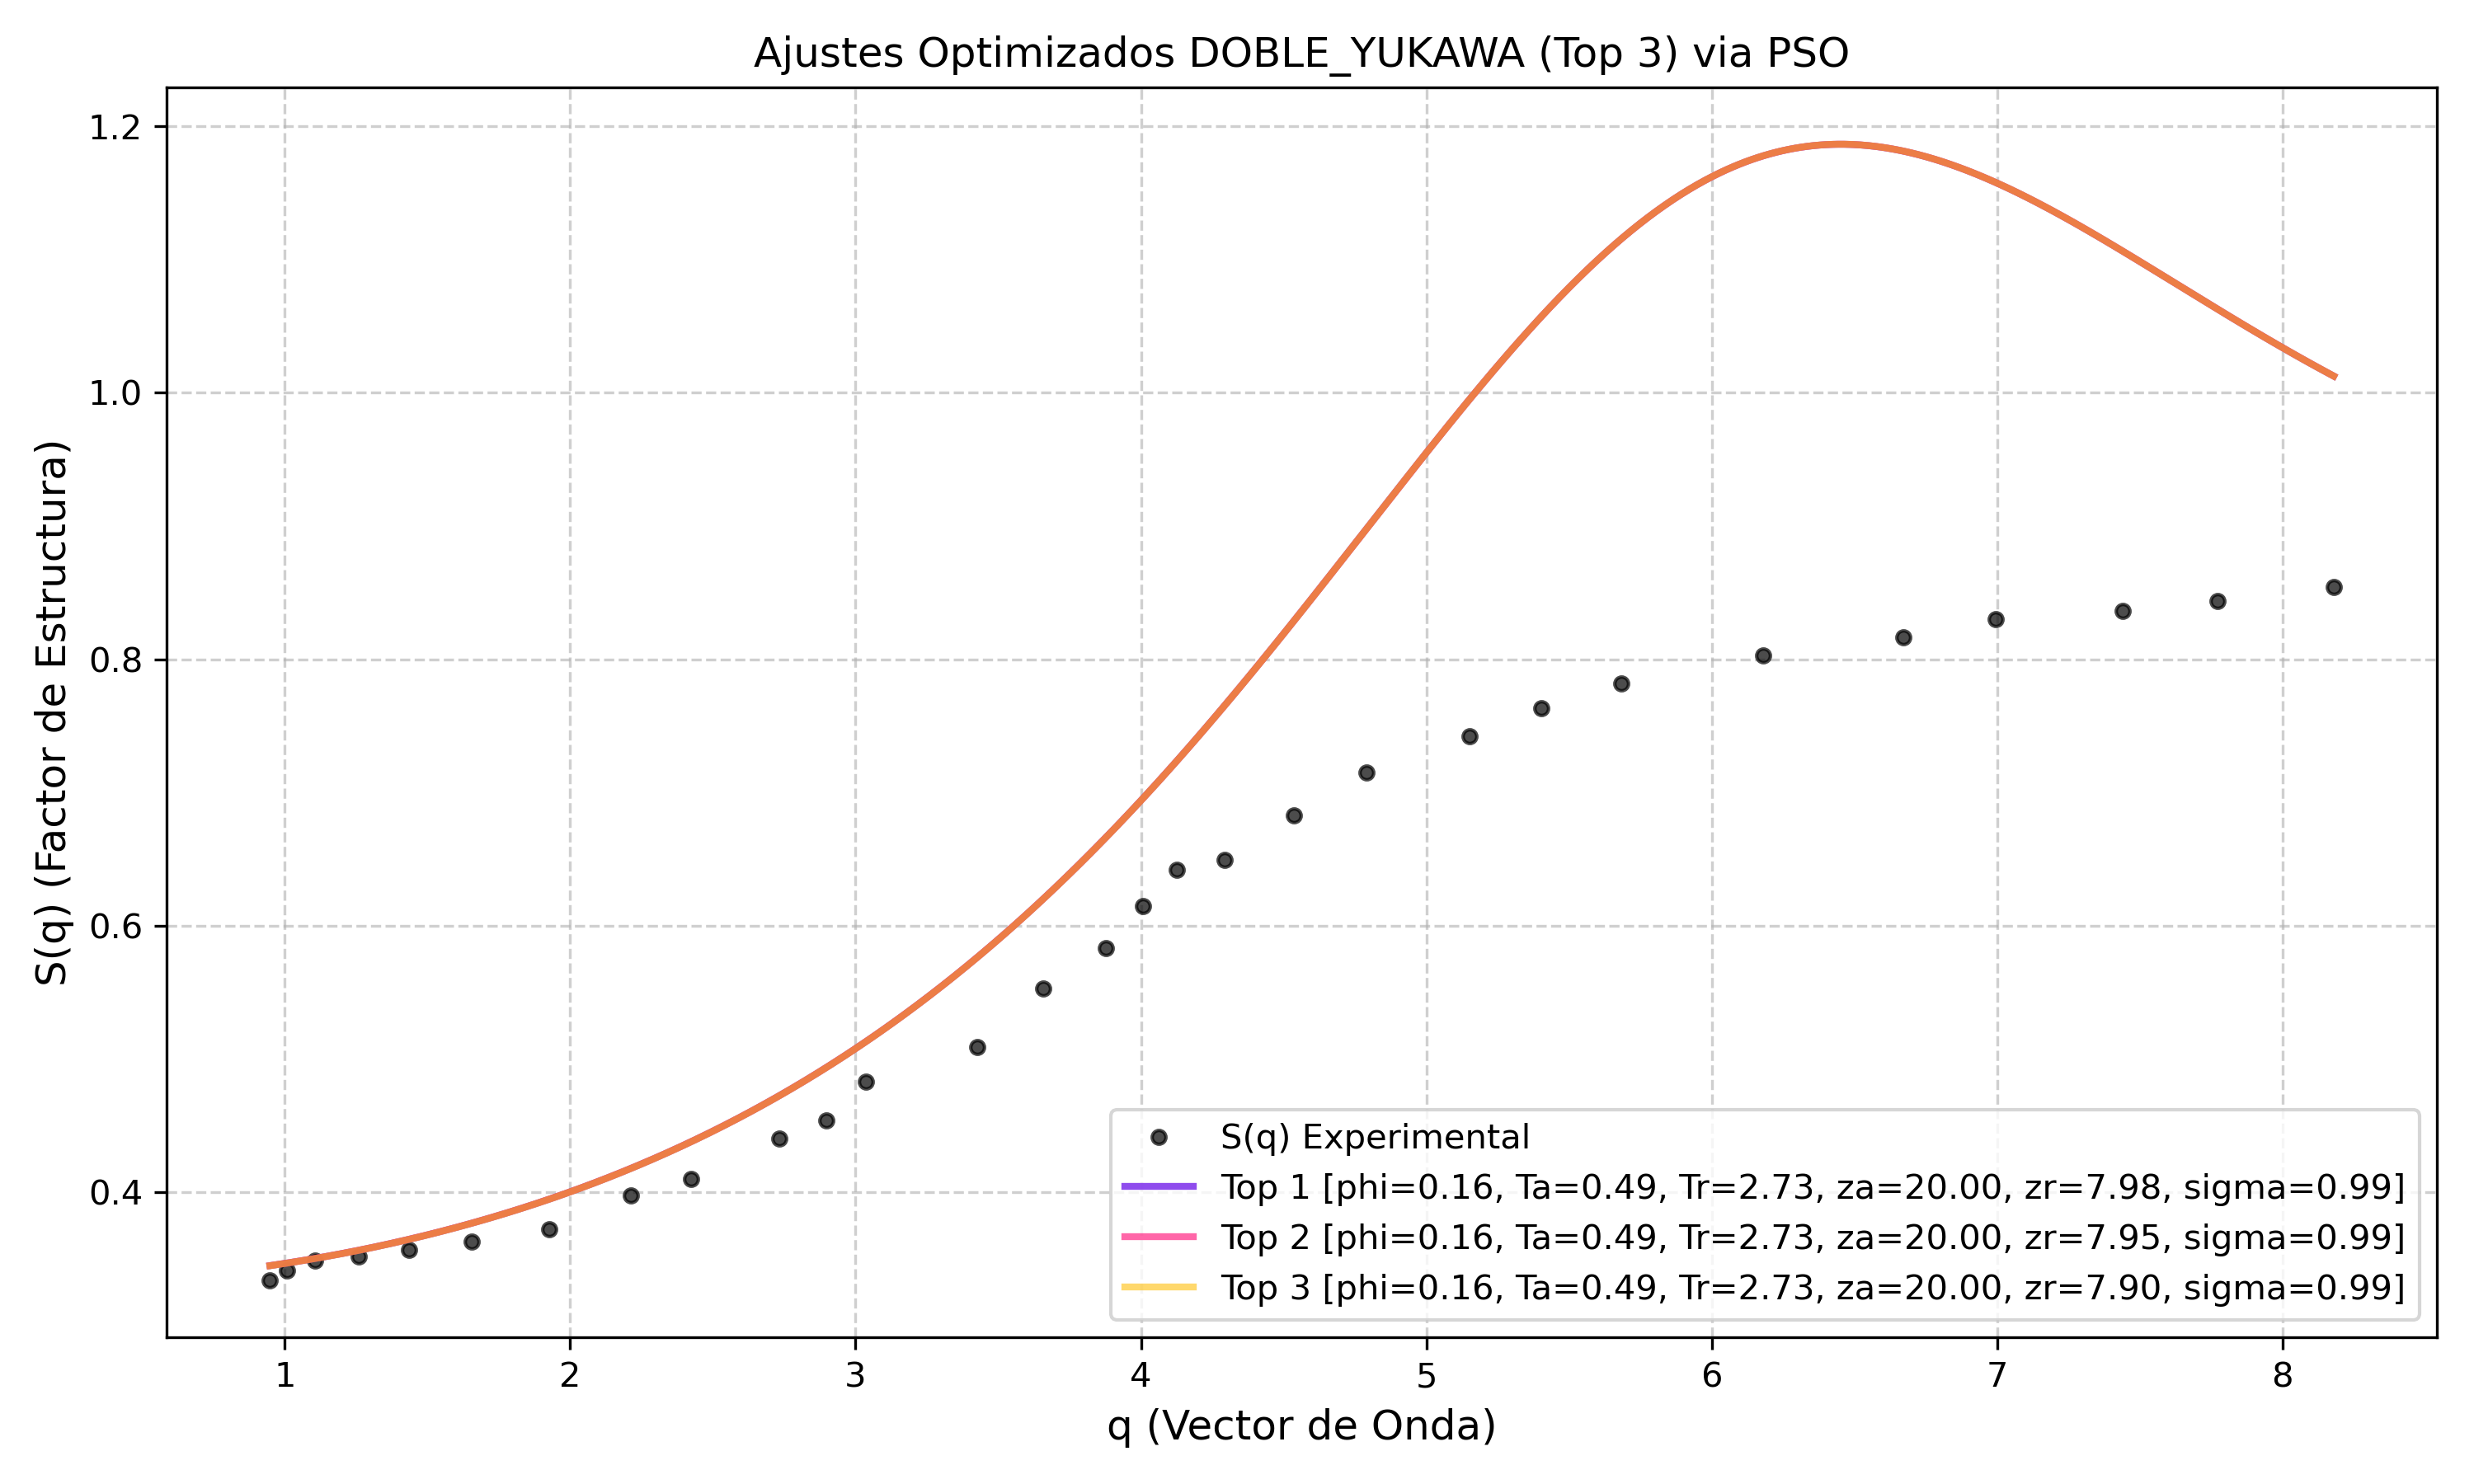
\includegraphics[width=0.8\textwidth]{plot_workflow_SmAb2:Arg.dat_pso.png}
\caption{Ajuste de los datos originales frente al top 3 continuo (PSO).}
\end{figure}
\vspace{0.5cm}
\hrule
\vspace{0.5cm}

\subsection*{Resultados para SmAb4:arg.dat\_pso (Modelo DOBLE_YUKAWA - PSO)}
\textbf{¿Cómo replicar?} Ejecute el siguiente comando en la terminal desde el directorio raíz:
\begin{verbatim}
python3 run_workflow.py Simulation_Data/SmAb4:arg.dat doble_yukawa pso
\end{verbatim}
\textbf{Algoritmo de Optimización:} Se utilizó PSO para la exploración del espacio de parámetros. \newline
\textbf{Límites de Búsqueda (Bounds):} Los parámetros variables fueron explorados dentro de los siguientes radios: \newline
phi $\in$ [0.01, 0.3], Ta $\in$ [0.1, 5.0], Tr $\in$ [0.1, 5.0], za $\in$ [0.01, 20.0], zr $\in$ [0.01, 20.0], sigma $\in$ [0.99, 1.01]
\vspace{0.4cm}
 
\begin{table}[h!]
\centering
\begin{tabular}{cccccccc}
\toprule
\textbf{Rango} & \textbf{phi} & \textbf{Ta} & \textbf{Tr} & \textbf{za} & \textbf{zr} & \textbf{sigma} & \textbf{Costo (MSE)} \\
\midrule
Top 1 & 0.168 & 0.310 & 0.100 & 20.000 & 17.061 & 0.990 & 0.01153 \\
Top 2 & 0.168 & 0.310 & 0.100 & 20.000 & 17.068 & 0.990 & 0.01153 \\
Top 3 & 0.168 & 0.310 & 0.100 & 20.000 & 17.055 & 0.990 & 0.01153 \\
\bottomrule
\end{tabular}
\caption{Parámetros top 3 obtenidos mediante PSO para este dataset.}
\end{table}
\begin{figure}[h!]
\centering
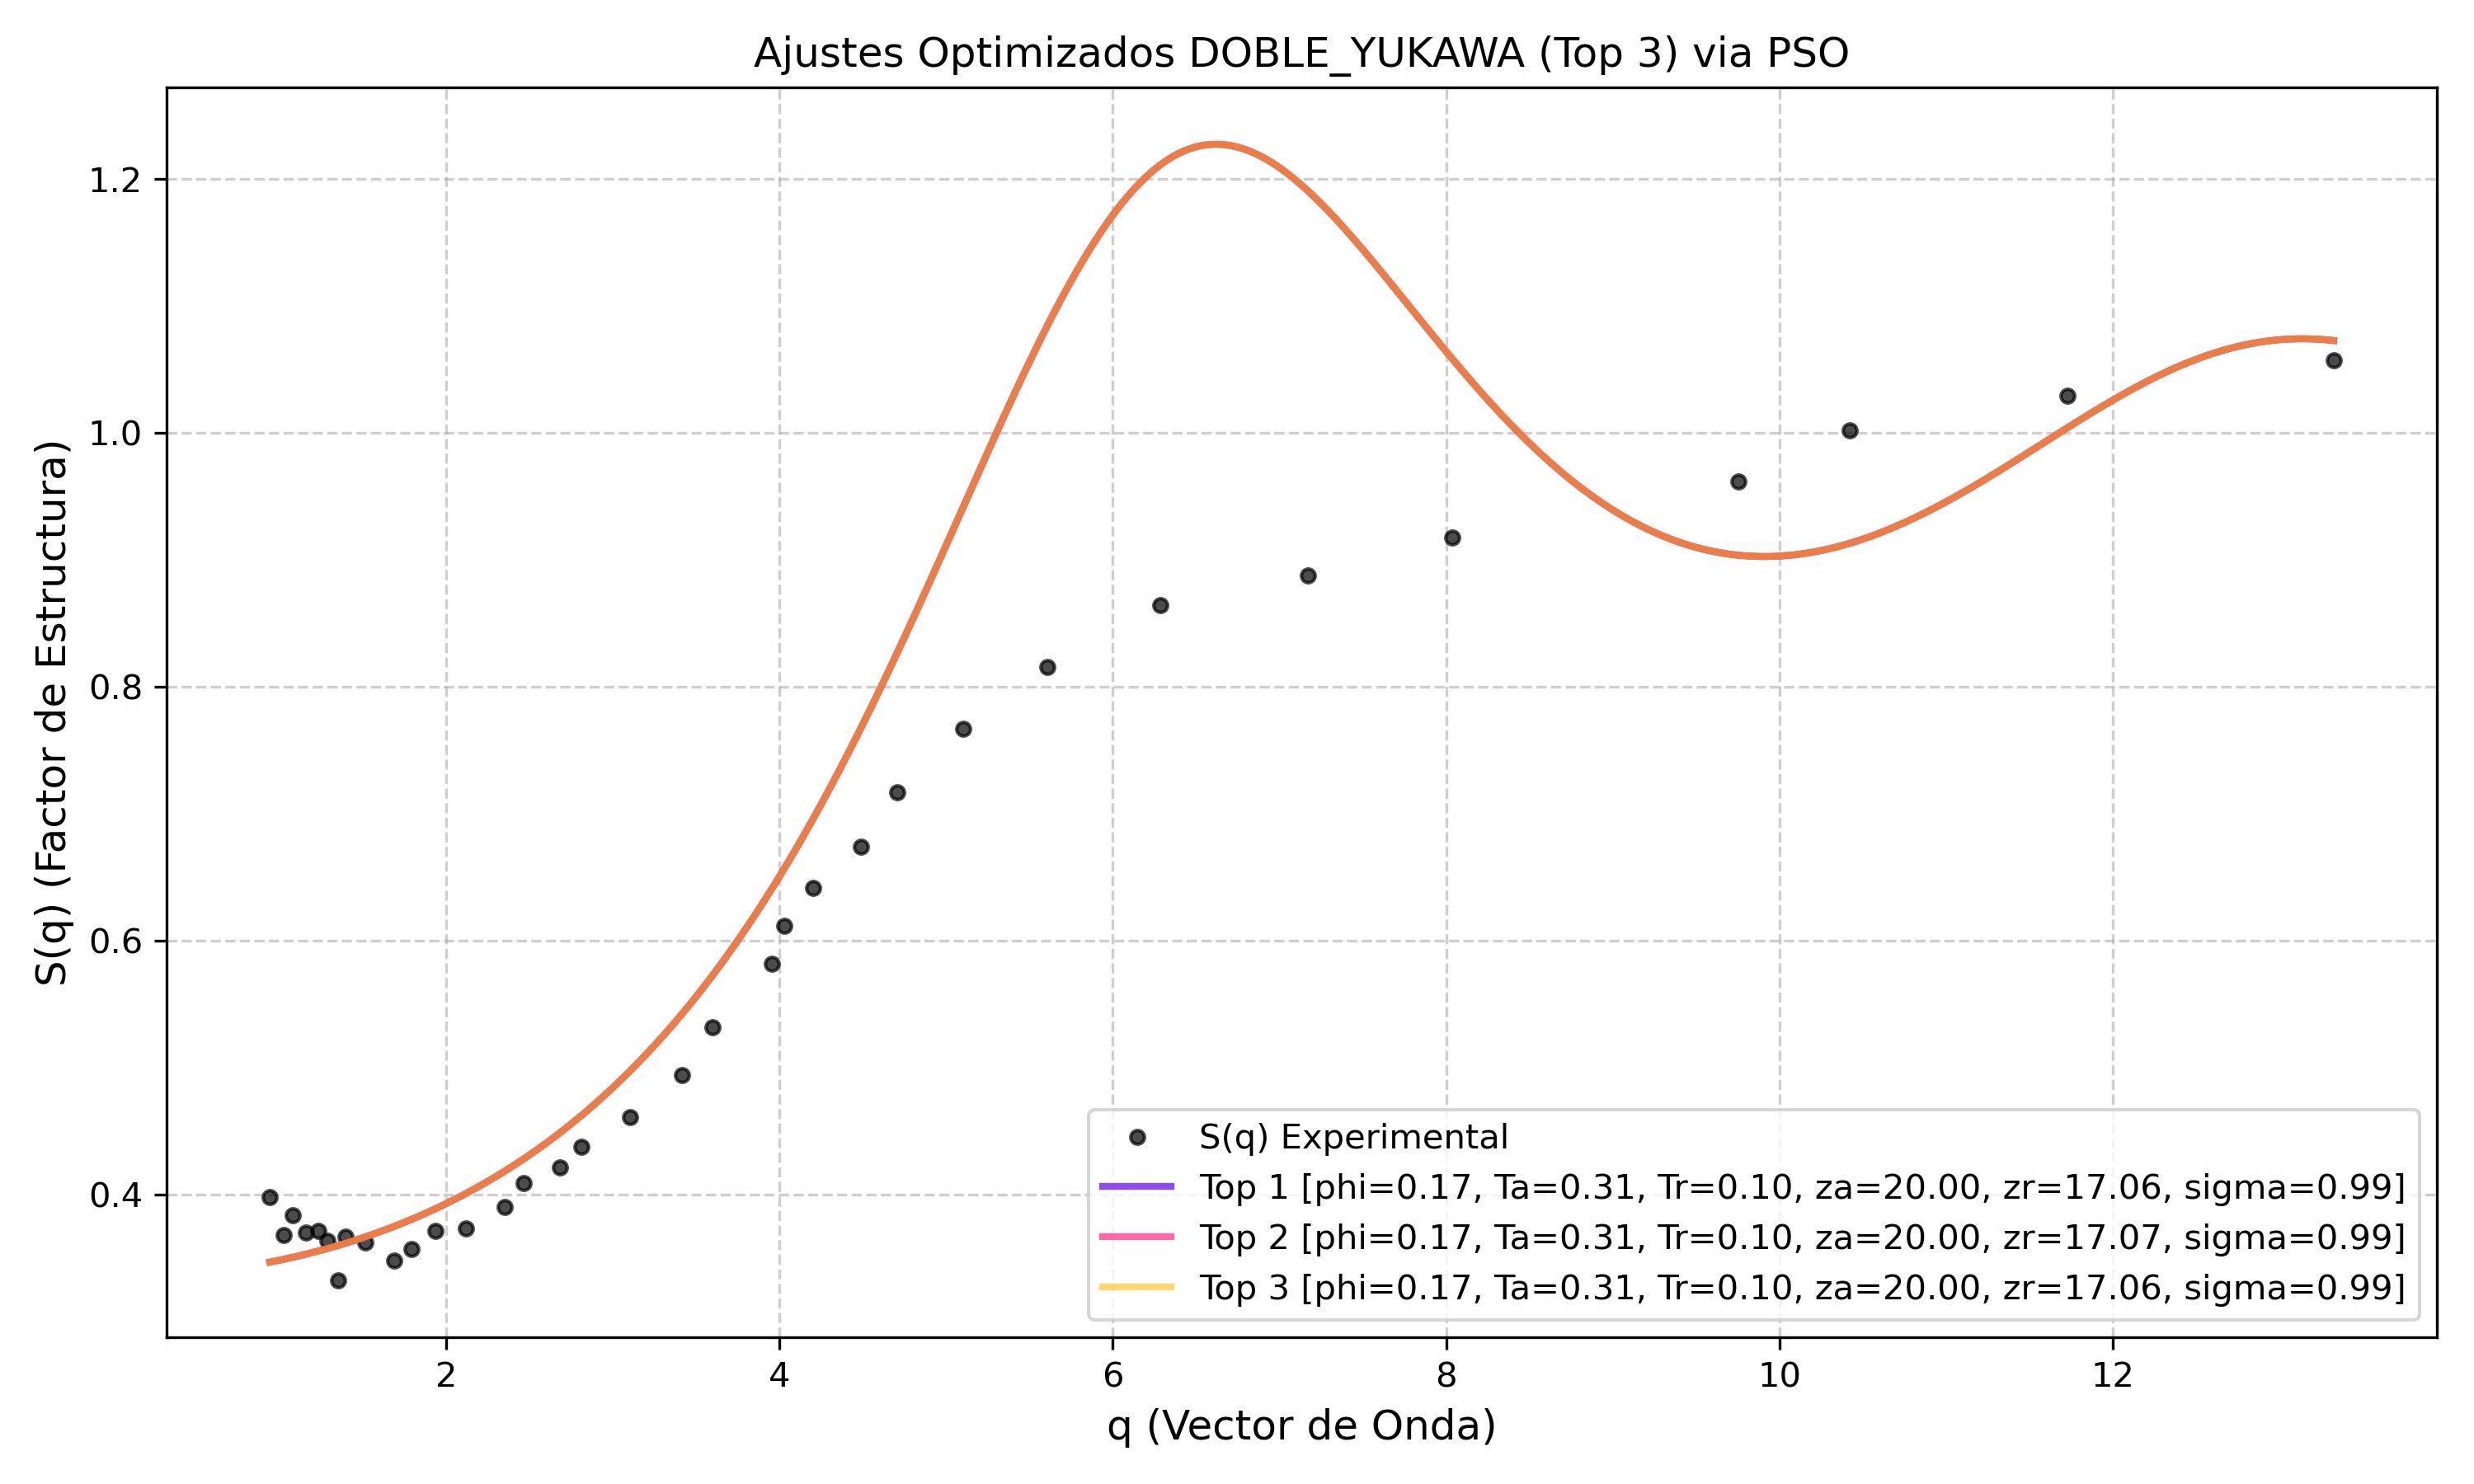
\includegraphics[width=0.8\textwidth]{plot_workflow_SmAb4:arg.dat_pso.png}
\caption{Ajuste de los datos originales frente al top 3 continuo (PSO).}
\end{figure}
\vspace{0.5cm}
\hrule
\vspace{0.5cm}

\subsection*{Resultados para SmAb2:NaCl.dat\_de (Modelo DOBLE_YUKAWA - DE)}
\textbf{¿Cómo replicar?} Ejecute el siguiente comando en la terminal desde el directorio raíz:
\begin{verbatim}
python3 run_workflow.py Simulation_Data/SmAb2:NaCl.dat doble_yukawa de
\end{verbatim}
\textbf{Algoritmo de Optimización:} Se utilizó DE para la exploración del espacio de parámetros. \newline
\textbf{Límites de Búsqueda (Bounds):} Los parámetros variables fueron explorados dentro de los siguientes radios: \newline
phi $\in$ [0.01, 0.3], Ta $\in$ [0.1, 5.0], Tr $\in$ [0.1, 5.0], za $\in$ [0.01, 20.0], zr $\in$ [0.01, 20.0], sigma $\in$ [0.99, 1.01]
\vspace{0.4cm}
 
\begin{table}[h!]
\centering
\begin{tabular}{cccccccc}
\toprule
\textbf{Rango} & \textbf{phi} & \textbf{Ta} & \textbf{Tr} & \textbf{za} & \textbf{zr} & \textbf{sigma} & \textbf{Costo (MSE)} \\
\midrule
Top 1 & 0.146 & 0.138 & 1.178 & 19.997 & 12.869 & 0.990 & 0.00462 \\
Top 2 & 0.148 & 0.139 & 1.190 & 20.197 & 12.998 & 1.000 & 0.00508 \\
Top 3 & 0.145 & 0.136 & 1.167 & 19.797 & 12.741 & 0.980 & 0.00485 \\
\bottomrule
\end{tabular}
\caption{Parámetros top 3 obtenidos mediante DE para este dataset.}
\end{table}
\begin{figure}[h!]
\centering
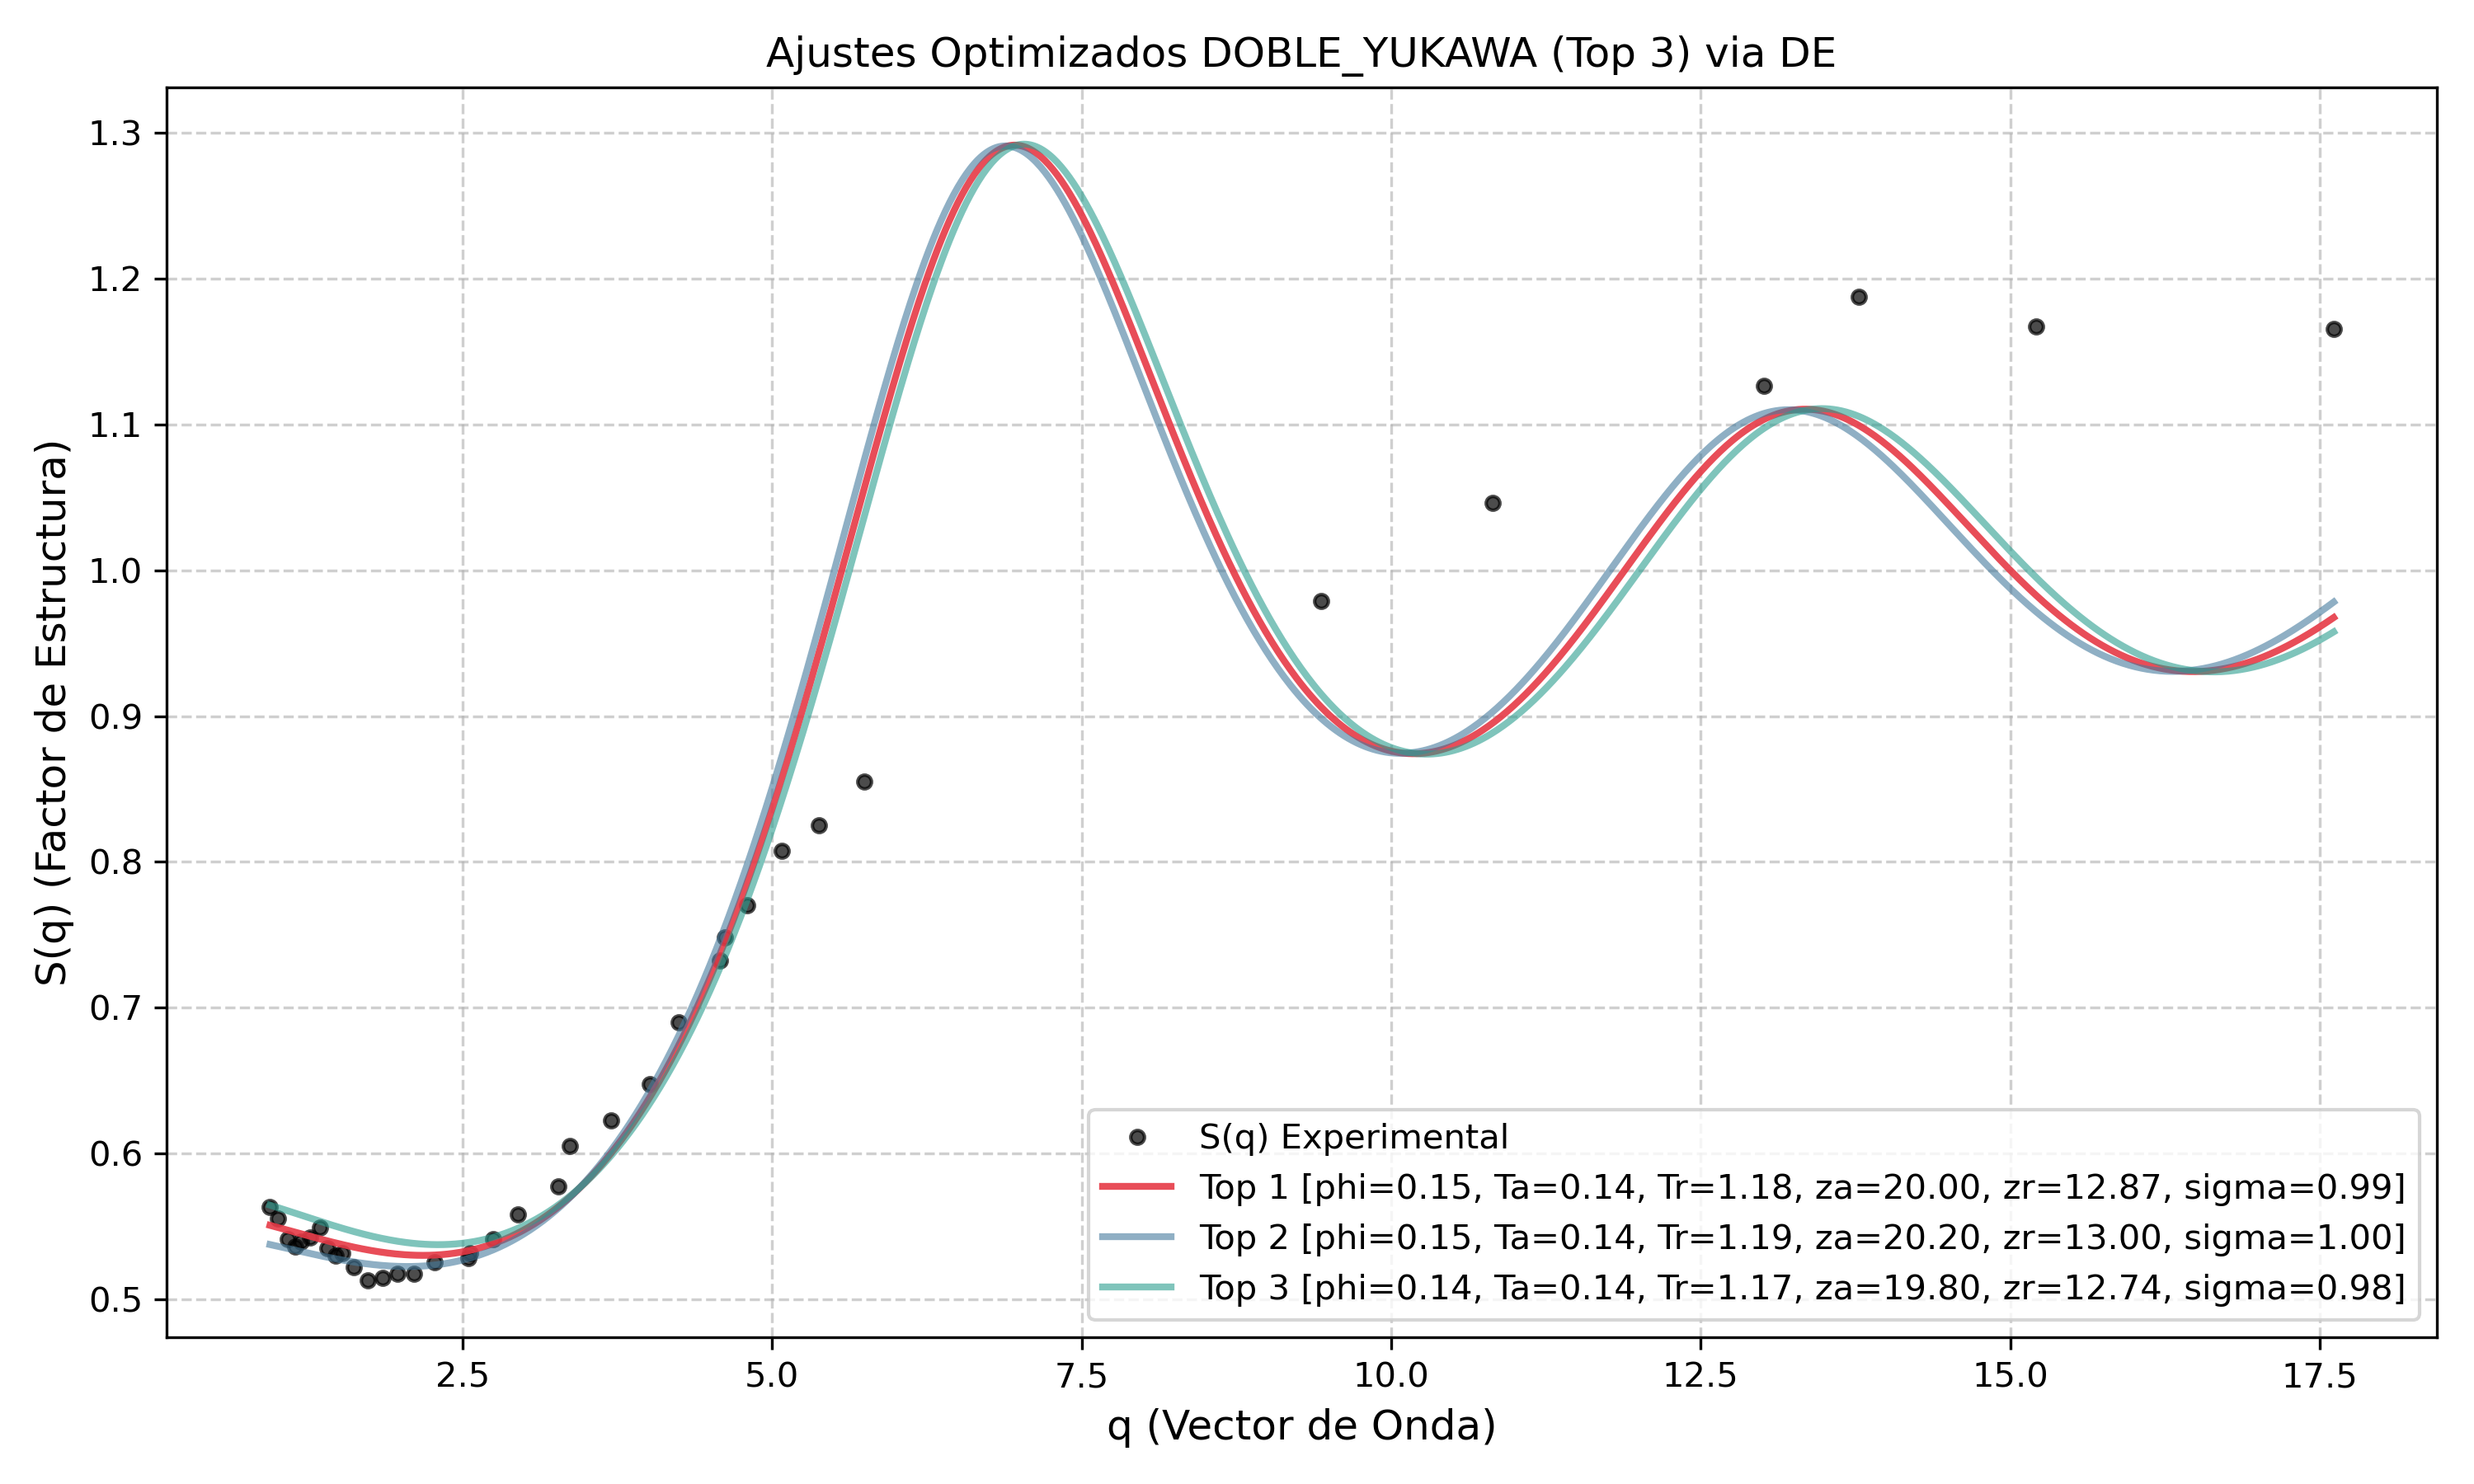
\includegraphics[width=0.8\textwidth]{plot_workflow_SmAb2:NaCl.dat_de.png}
\caption{Ajuste de los datos originales frente al top 3 continuo (DE).}
\end{figure}
\vspace{0.5cm}
\hrule
\vspace{0.5cm}

\subsection*{Resultados para SmAb4:NaCl.dat\_de (Modelo DOBLE_YUKAWA - DE)}
\textbf{¿Cómo replicar?} Ejecute el siguiente comando en la terminal desde el directorio raíz:
\begin{verbatim}
python3 run_workflow.py Simulation_Data/SmAb4:NaCl.dat doble_yukawa de
\end{verbatim}
\textbf{Algoritmo de Optimización:} Se utilizó DE para la exploración del espacio de parámetros. \newline
\textbf{Límites de Búsqueda (Bounds):} Los parámetros variables fueron explorados dentro de los siguientes radios: \newline
phi $\in$ [0.01, 0.3], Ta $\in$ [0.1, 5.0], Tr $\in$ [0.1, 5.0], za $\in$ [0.01, 20.0], zr $\in$ [0.01, 20.0], sigma $\in$ [0.99, 1.01]
\vspace{0.4cm}
 
\begin{table}[h!]
\centering
\begin{tabular}{cccccccc}
\toprule
\textbf{Rango} & \textbf{phi} & \textbf{Ta} & \textbf{Tr} & \textbf{za} & \textbf{zr} & \textbf{sigma} & \textbf{Costo (MSE)} \\
\midrule
Top 1 & 0.115 & 1.216 & 3.208 & 1.763 & 4.154 & 0.990 & 0.03754 \\
Top 2 & 0.116 & 1.228 & 3.240 & 1.781 & 4.196 & 1.000 & 0.04130 \\
Top 3 & 0.114 & 1.204 & 3.175 & 1.745 & 4.112 & 0.980 & 0.03942 \\
\bottomrule
\end{tabular}
\caption{Parámetros top 3 obtenidos mediante DE para este dataset.}
\end{table}
\begin{figure}[h!]
\centering
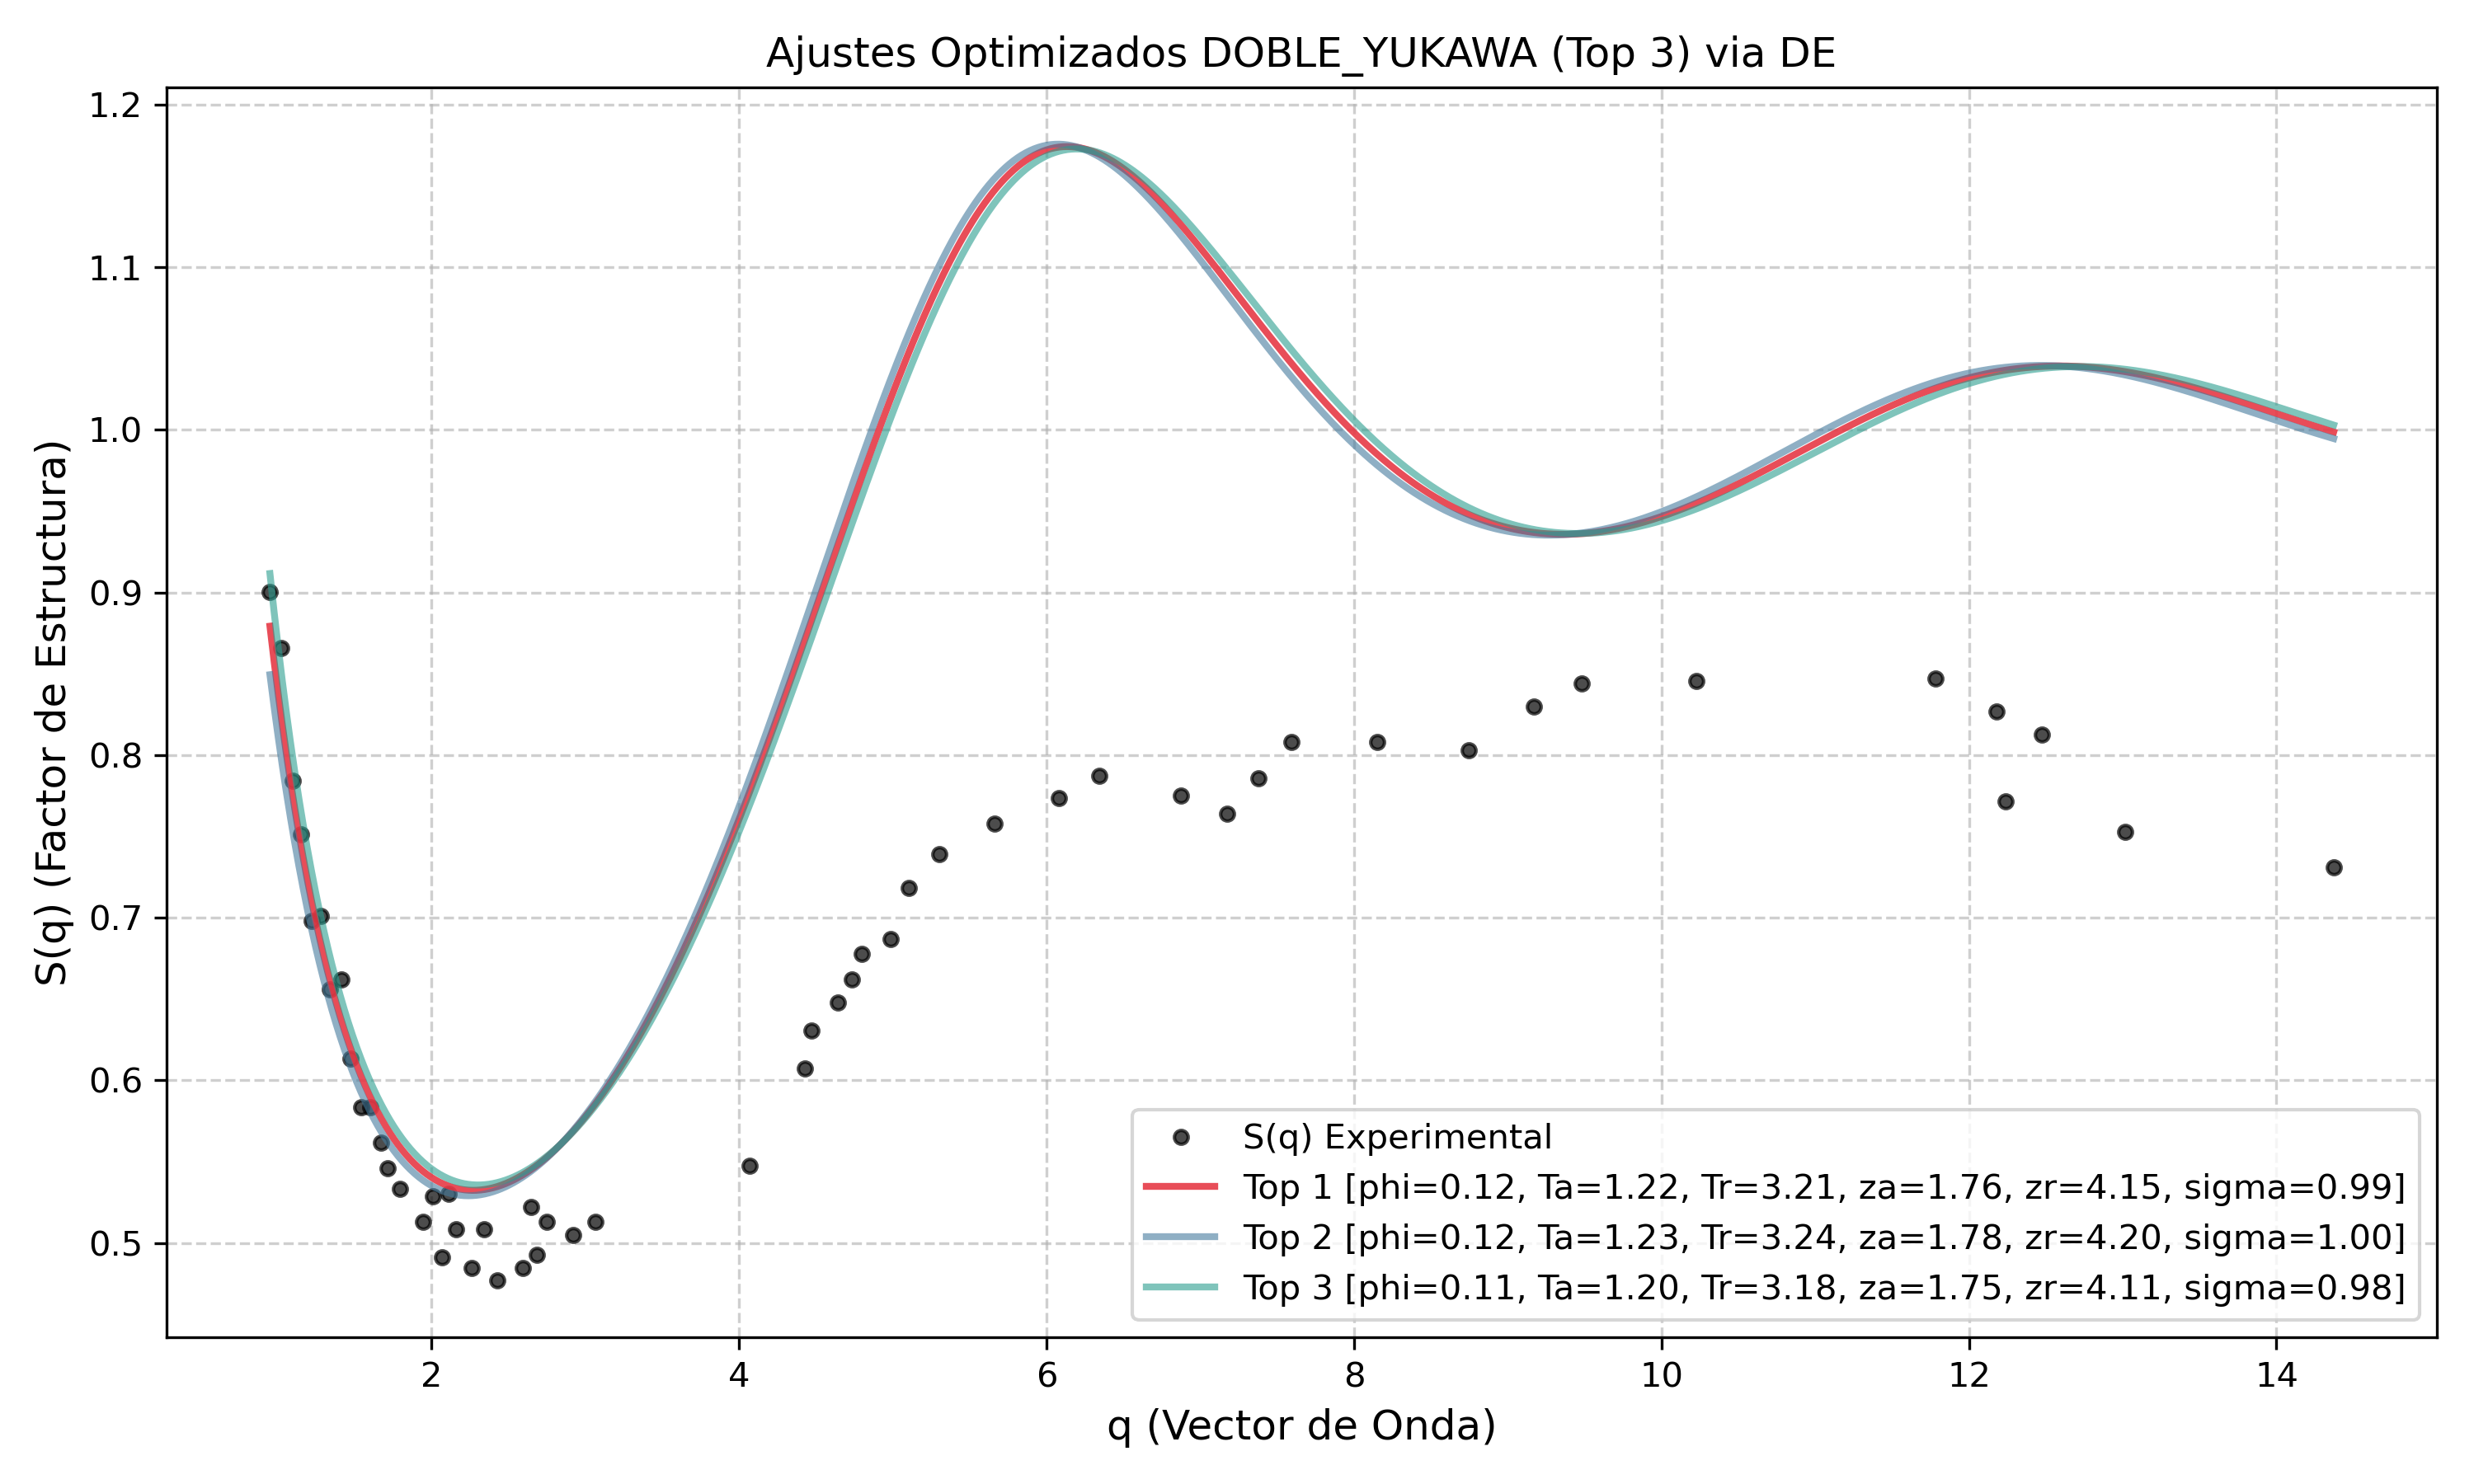
\includegraphics[width=0.8\textwidth]{plot_workflow_SmAb4:NaCl.dat_de.png}
\caption{Ajuste de los datos originales frente al top 3 continuo (DE).}
\end{figure}
\vspace{0.5cm}
\hrule
\vspace{0.5cm}

%%APPEND_RESULTS_HERE%%

\section{Conclusiones}
La infraestructura automatizada logró exitosamente un ajuste para inferir los parámetros subyacentes del factor de estructura estático en una fase totalmente desatendida, confirmándose la flexibilidad de ensamblar un backend eficiente en C con la estrategia de Evolución Diferencial comandada desde Python.

\end{document}
